
%\newpage
\newcommand{\blinks}{\{links\}}
% François Version 2: 
%\section{Extending access to new types of data products  in ObsTAP services}\label{sec:accessoptions}
%\section{Possible Approaches for Accessing \gls{HEA} Data Products Using ObsTAP Services}\label{sec:accessoptions}
%\section{Access methods for data related to sky datasets discovered with ObsTAP}
%(Various implementation strategies for data access)

%\subsection{Difference between hea-event-list, hea-event-bundle, response function and analysis data products}
%As discussed in the previous section, high energy data distribution requires a special focus on event lists and associated response functions as well as analysis data products. 
%Event lists without corresponding response functions do not allow data interpretation. That’s the reason why hea-event-lists are often gathered in the same package with the response function in an “hea-event-bundle” with a specific format (OGIP, GADF or VODF).  In addition, the High Energy astronomical community has developed a lot of probabilistic analysis methods to analyse and extract information  from the event lists.  They cannot all be described by ObsCore parameters due to the richness and  complexity of their parameters. They are listed in section~\ref{sec:voc_product_type}. Access to this category of data can be managed similarly to response functions in some cases, as proposed in section \ref{sec:analysis-dp}.

As discussed previously, \gls{HEA} data distribution requires special focus on event lists and their associated \glspl{IRF}, as well as on advanced data products.  In most cases, corresponding \glspl{IRF} are required to enable physical interpretation of event list data, at least for some physical axes.  That is one reason why data providers may prefer to package an {\bf hea-event-list} together with the associated {\bf response-function}s, or with other ancillary data products that enable end-users to construct appropriate \glspl{IRF}, in a single package.  We have proposed an {\bf hea-event-bundle} data product type to represent such packages, which may be recorded in a specific format such as OGIP FITS, GADF FITS, or VODF FITS, or may simply consist of a set of data products in a common archive file format such as a tarball.

In other cases, recognizing the computation complexity of analyzing \gls{HEA} data robustly in the extreme Poisson regime, \gls{HEA} data providers may choose to provide advanced data products, such as probability density functions or statistical draws, directly to the user community.  In most cases, these advanced data products have spatial, spectral, and/or temporal coverage that can be directly described using standard ObsCore attributes, and therefore these data products can be discovered directly.  In other cases, these data products may not be describable using standard ObsCore parameters, either due to the richness and complexity of their parameters or because they depend on non-sky based parameters ({\em e.g.\/}, telescope altitude and azimuth).
%%-  Access to this category of data may be managed similarly to {\bf response-function}s in some cases, as proposed in section \ref{sec:analysis-dp}.

In this section, we first discuss direct access to individual \gls{HEA} data products (including an {\bf hea-event-bundle}), and then focus on several possible approaches that use DataLink \citep{2023ivoa.spec.1215B} to facilitate access to additional datasets that may be associated with a primary datasets ({\em e.g.\/}, {\bf response-function}s associated with a primary {\bf hea-event-list}). Finally, we discuss the use of one or more additional tables joined with the {\tt ivoa.obscore} table as a means to access certain types of data products.

The choice of access method is up to the data provider.

If a data collection consists primarily of individual observations, each with a small set of associated data products such as \glspl{IRF} that are required for further data analysis (this is a very common use case), then either direct access to the {\bf hea-event-bundle}s or access via DataLink is generally preferable.

However, if the data collection includes data products such as spectra, light-curves, or advanced data products ({\em e.g.\/}, aperture photometry probability density functions) that are extracted from the primary {\bf hea-event-list} and that can be used independently of the primary dataset, then direct access to these products is likely preferable from the user's perspective.  Since \gls{HEA} event lists typically simultaneously encode spatial, spectral, and temporal information, a very large amount of data may be associated with a single {\bf hea-event-list}.  For example, roughly 4,600 individual detectable X-ray sources are located in a single deep Chandra observation field of view centered on the Galactic center.  Using DataLink to the primary {\bf hea-event-list} to access these spectra, light-curves, and advanced data products would be unwieldy, especially when only a small subset of the products are required.

Direct access and access via DataLink to X-ray (Chandra X-ray Observatory)\footnote{\url{https://wiki.ivoa.net/internal/IVOA/InterOpJune2026HEIG/EvansI_ObsCore_HEA_Demo.pptx}.}, Gamma ray (Cherenkov Telescope Array Observatory)\footnote{\url{https://wiki.ivoa.net/internal/IVOA/InterOpJune2026HEIG/CTAO-HESS_Data_Access_-_Servillat_-_2026-06-09.pdf}.}, and particle astrophysics (MK3NeT neutrino telescope)\footnote{\url{https://wiki.ivoa.net/internal/IVOA/InterOpJune2026HEIG/2026_06_IVOA_interop_Strasbourg_neutrino_use_case.pptx.pdf}.} data products was demonstrated at the IVOA June 2026 Interoperability meeting using prototype implementations of the enhancements to current IVOA standards proposed in this document.

\subsection{Direct Access to a Data Product or {\bf hea-event-bundle}}
% The simplest method to access hea-event-list and associated response function is to provide a link to an hea-event-bundle package; this can be done by providing an URL to the package in the {\em access\_url \/} FIELD of the ObsCore (or ObsCore + extension) table. The {\em access\_format \/} FIELD will contain the appropriate MIME type for the bundle package (for example x-fits-ogip, x-fits-gadf, or x-fits-vodf). Table~\ref{tab:bundle} shows an excerpt of an ObsCore result and illustrates this method. This method  can be combined with methods described below in~\ref{sec:datalink} for a common access to the bundle and other resources such as previews or some specific analysis data products.

The simplest method to directly access any data product is to provide a direct link to the data product.  This can be done by providing a URL to the product in the {\em access\_url\/} attribute of the ObsCore table. The {\em access\_format\/} attribute will contain the appropriate MIME type for the data product ({\em e.g.\/}, {\tt x-fits-bintable}).  In the case of an {\bf hea-event-list} together with associated data products such as \glspl{IRF}, a link to an {\bf hea-event-bundle} package may be provided.  In this case, the {\em access\_format \/} attribute will contain the appropriate MIME type for the bundle package ({\em e.g.\/}, {\tt x-fits-ogip}, {\tt x-fits-gadf\/}, {\tt x-fits-vodf}, {\tt application/x-tar}). Table~\ref{tab:bundle} shows an excerpt of an ObsCore result that illustrates this approach. This method  can be combined with methods described below in \S~\ref{sec:datalink} for common access to the bundle and other resources such as previews or some specific advanced data products.

%\begin{landscape}
\begin{longtable}{|m{0.22\linewidth}|m{0.34\linewidth}|m{0.34\linewidth}|}
\hline
{\bf Attribute}&{\bf Row 1 Value}&{\bf Row 2 Value}\\
%\hline
\hline
{\em dataproduct\_type\/}& {\tt hea-event-bundle}&{\tt hea-event-bundle}\\
\hline
%{\em dataproduct\_subtype\/}&{\tt GADF DL3}&{\tt GADF DL3}\\
%\hline
{\em calib\_level\/}& 2&2\\
\hline
{\em obs\_collection\/}& HESS-DL3-DR1&HESS-DL3-DR1\\
\hline
{\em obs\_id\/}&20136&20317\\
\hline
{\em access\_url\/}& \footnotesize{https://hess-dr.obspm.fr/\newline retrieve/hess\_dl3\_dr1\_obs\newline\_id\_020136.fits.gz}&\footnotesize{https://hess-dr.obspm.fr/\newline retrieve/hess\_dl3\_dr1\_obs\newline\_id\_020137.fits.gz}\\
\hline
{\em access\_format\/}&x-fits-gadf&x-fits-gadf\\
\hline
{\em access\_estsize\/}&414720&216000\\
\hline
\caption{Excerpt of the ObsCore Response for {\bf hea-event-bundle}s (Inspired by the \gls{HESS} ObsTAP Prototype at Paris Observatory).}
\label{tab:bundle}
\end{longtable}
%\end{landscape}

\subsection{Access via DataLink}
\label{sec:datalink}


DataLink \citep{2023ivoa.spec.1215B} allows a data provider to relate a main record provided by a service (ObsTAP, SSA/SIA, or a catalog service) to a arbitrary set of links that complement the information contained in the record. An implementation note \citep{2024ivoa.note.datalink} provides some hints on how to use this standard.
There are at least three ways to implement this standard for {\bf hea-event-list}s depending how many steps are used in the access method to the associated datasets:
 \begin{itemize}
	\item Subsection~\ref{sec:datalinkinobs} outlines the standard two-step approach;
	\item Subsection~\ref{sec:datalinksd} demonstrates both direct access to the {\bf hea-event-list} and two-step access to the additional material;
 	\item Subsection~\ref{sec:datalinktap} allows direct access to both the {\bf hea-event-list} plus additional data products, such as \glspl{IRF} or advanced data products.  This approach is not described in the DataLink standard but is fully consistant with TAP and the DataLink \blinks\ endpoint response specification.
 \end{itemize}
	 
\subsubsection{From an {\bf hea-event-list} in ObsCore: DataLink to Access the Event List and Response Functions via {\em access\_url\/}}
\label{sec:datalinkinobs}
The {\em dataproduct\_type\/} exposed in ObsCore is {\bf hea-event-list} and the Data\-Link \blinks\ endpoint response  points to the event list and to the various {\bf response-function}s individually. This solution allows retrieval of data with explicit access to the various  components  of a ``bundle,'' which doesn't need to be packaged in that case. In addition to \glspl{IRF}, additional data products, including advanced data products, can also be linked to the {\bf hea-event-list} this way.
% Figure~\ref{fig:obscoretodl} shows an ObsCore response where the selected record points to a \blinks\ endpoint response illustrating this method.
Table~\ref{tab:datalink} provides example DataLink response content to a query for \gls{HESS} Data Level 3 Public Test Data.
%\begin{figure}
%
%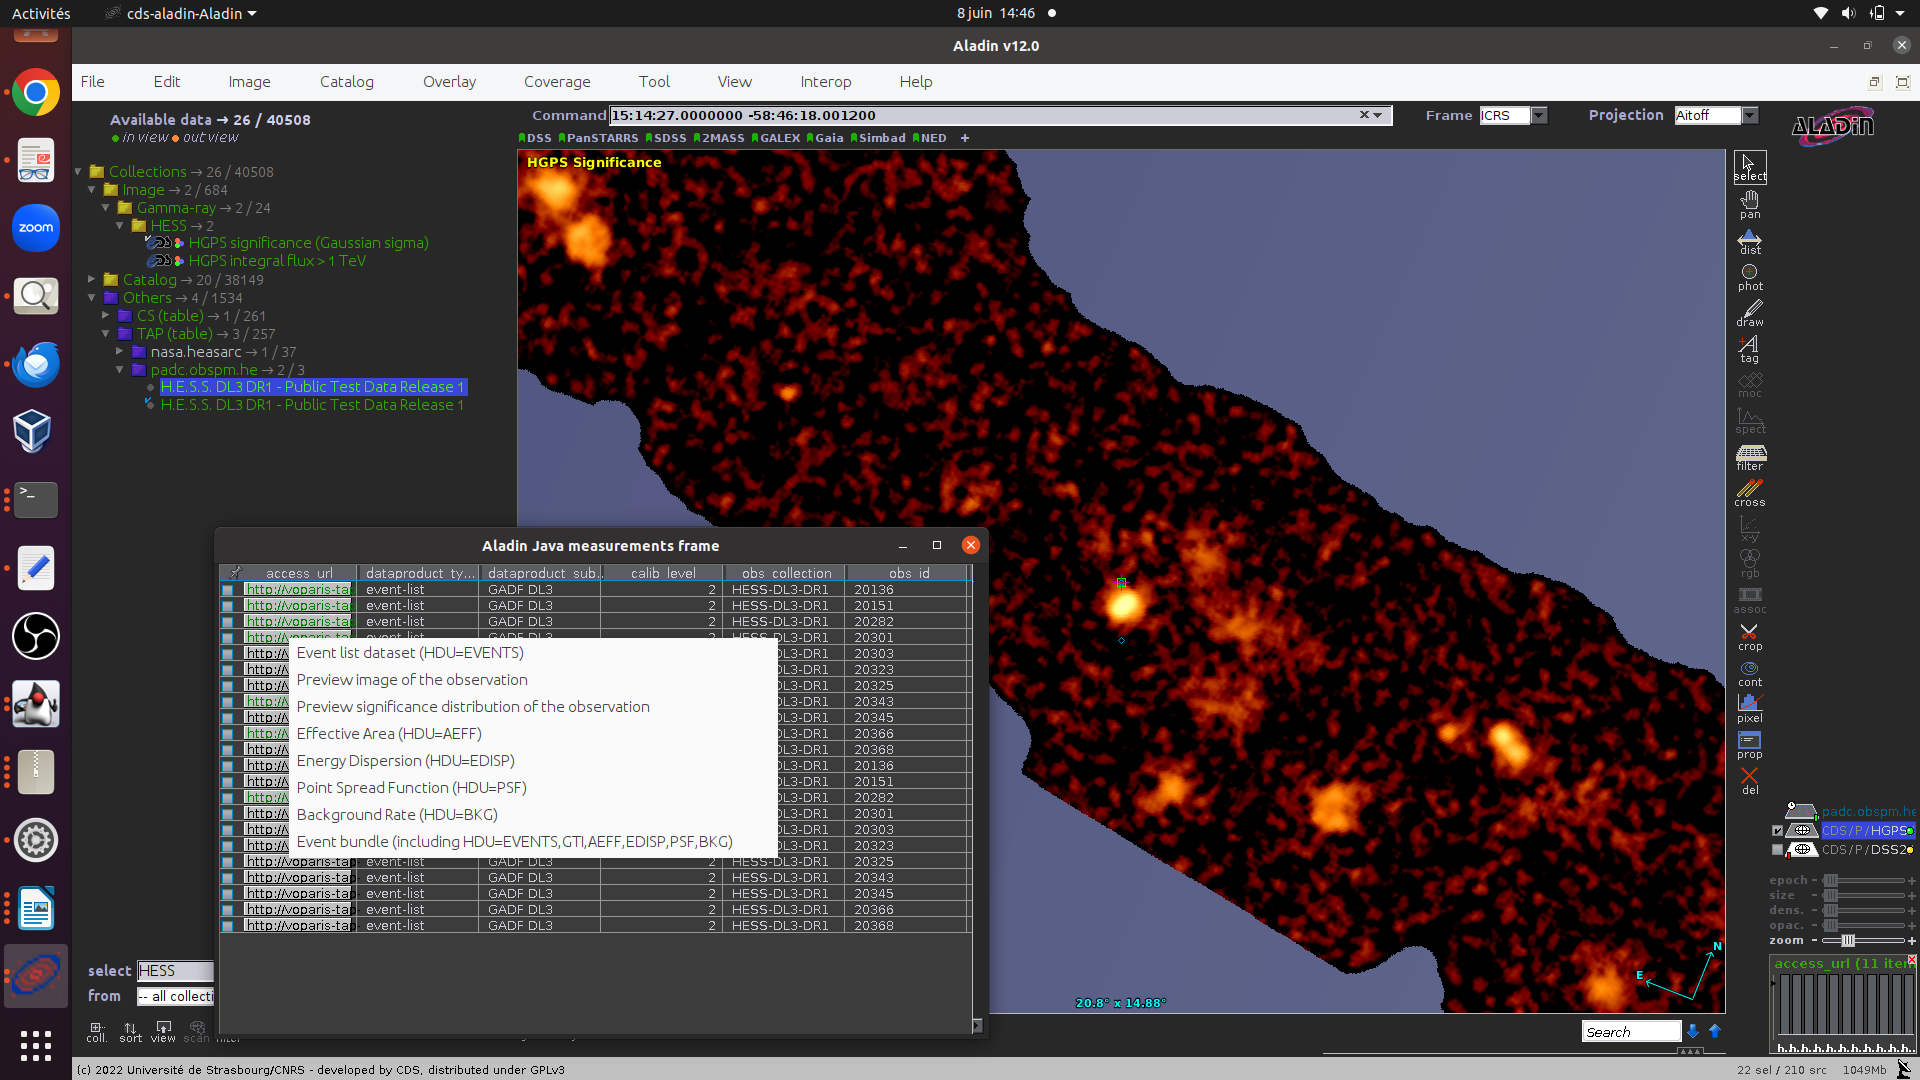
\includegraphics[width=1.5\textwidth, angle=90]{Obscore+datalink.png}
% \caption{Selection of H.E.S.S. data from Aladin Desktop: In the galactic center area, an ObsTAP query has been performed and H.E.S.S. datasets are discovered.  One of the ObsCore record has been selected and points to a DataLink response, with 8 links provided in the white box. The content of this DataLink table is described in Table~\ref{tab:datalink}. }
%\label{fig:obscoretodl}
%\end{figure}

\begin{landscape}
\begin{center}
\begin{longtable}{|m{0.08\linewidth}|m{0.3\linewidth}|m{0.08\linewidth}|m{0.22\linewidth}|m{0.1\linewidth}|m{0.14\linewidth}|m{0.13\linewidth}|}
\hline%\sptablerule
\textbf{ID}  &\textbf{\footnotesize access\_url}  &\textbf{\footnotesize semantics}&\textbf{\footnotesize description} &\textbf{\footnotesize content\_type}  &\textbf{\footnotesize content\_qualifier}\cr
\hline%\sptablerule
{\footnotesize 20136} & {\footnotesize https://hess-dr.obspm.fr/retrieve/hess\_dl3\newline \_dr1\_obs\_id\_020136.fits.gz\#EVENTS} & {\footnotesize \#this} & {\footnotesize Event list dataset\newline (HDU=EVENTS) } & {\footnotesize x-fits-gadf}  & {\footnotesize hea-event-list} \cr
\hline%\sptablerule
{\footnotesize 20136} & {\footnotesize https://hess-dr.obspm.fr/retrieve/hess\_dl3\newline \_dr1\_obs\_id\_020136\_image.png} & {\footnotesize \#preview-image} & {\footnotesize Preview image of the observation} & {\footnotesize image/png}  & {\footnotesize preview} \cr
\hline%\sptablerule
{\footnotesize 20136} & {\footnotesize https://hess-dr.obspm.fr/retrieve/hess\_dl3\newline \_dr1\_obs\_id\_020136\_plot.png} & {\footnotesize \#preview-plot} & {\footnotesize Preview significance distribution of the observation } & {\footnotesize image/png}  & {\footnotesize preview} \cr
\hline%\sptablerule
{\footnotesize 20136} & {\footnotesize https://hess-dr.obspm.fr/retrieve/hess\_dl3\newline \_dr1\_obs\_id\_020136.fits.gz\#AEFF } & {\footnotesize \#calibration} & {\footnotesize Effective Area (HDU=AEFF)}   & {\footnotesize x-fits-gadf}  & {\footnotesize aeff} \cr
\hline%\sptablerule
{\footnotesize 20316} & {\footnotesize https://hess-dr.obspm.fr/retrieve/hess\_dl3\newline \_dr1\_obs\_id\_020136.fits.gz\#EDISP} & {\footnotesize \#calibration} & {\footnotesize Energy Dispersion\newline (HDU=EDISP)} & {\footnotesize x-fits-gadf}  & {\footnotesize edisp} \cr
\hline%\sptablerule
{\footnotesize 20316} & {\footnotesize https://hess-dr.obspm.fr/retrieve/hess\_dl3\newline \_dr1\_obs\_id\_020136.fits.gz\#PSF} & {\footnotesize \#calibration} & {\footnotesize Point Spread Function\newline (HDU=PSF) } & {\footnotesize x-fits-gadf}  & {\footnotesize psf} \cr
\hline%\sptablerule
{\footnotesize 20316} & {\footnotesize https://hess-dr.obspm.fr/retrieve/hess\_dl3\newline \_dr1\_obs\_id\_020136.fits.gz\#BKG} & {\footnotesize \#calibration} & {\footnotesize Background Rate (HDU=BKG) }  & {\footnotesize x-fits-gadf}  & {\footnotesize bkgrate} \cr
\hline%\sptablerule
{\footnotesize 20316} & {\footnotesize https://hess-dr.obspm.fr/retrieve/hess\_dl3\newline \_dr1\_obs\_id\_020136.fits.gz} & {\footnotesize \#package} & {\footnotesize Event bundle (including\newline HDU=EVENTS,GTI,AEFF,\newline EDISP,PSF,BKG)  }  & {\footnotesize x-fits-gadf}  & {\footnotesize hea-event-bundle } \cr
\hline%\sptablerule

\caption{DataLink Response Table Attached to an {\bf hea-event-list}  record in ObsCore. Inspired from Paris Observatory \gls{HESS} ObsTAP Prototype.}
\label{tab:datalink}
\end{longtable}
\end{center}
\end{landscape}

\subsubsection{Datalink Access Using a Service Descriptor}
\label{sec:datalinksd}
To avoid preventing a direct access to the {\bf hea-event-list} while keeping the explicit access to the various response functions, one can add a ``DataLink'' service descriptor in the ObsTAP result as shown in the example below.

{\small
\begin{verbatim}
<RESOURCE name="datalink" type="meta" utype="adhoc:service">
<DESCRIPTION>Datalink service</DESCRIPTION>
<PARAM arraysize="*" datatype="char" name="standardID"
   	value="ivo://ivoa.net/std/datalink#links-1.1"/>
<PARAM arraysize="*" datatype="char" name="accessURL"
   	value="http:/provider.org/dataservice/datalink"/>
<GROUP name="inputParams">
<PARAM name="ID" datatype="char" arraysize="*" value=""
   	ref="referenced_ID_FIELD"/></GROUP>
<PARAM arraysize="*" datatype="char" name="contentType"
   	value="application/x-votable+xml;content=datalink"/>
</RESOURCE>
\end{verbatim}
}

In this case the service descriptor provides the root URL to the DataLink \blinks\ endpoint. The full \blinks\ endpoint URL for a specific row (or group of rows) is built by adding the content of the referenced ID field this way:

\noindent {\tt http://provider.org/dataservice/datalink?ID={referenced\_ID\_field}}.

\noindent Note that the referenced ID field is not required to be  {\em obs\_publisher\_did\/}. It can be  {\em obs\_id\/}, or any free identifier attribute, allowing grouping of several rows together. For example, referencing {\em obs\_id\/} will allow all the datasets belonging to the same observation to be bound to the same \blinks\ endpoint response.
      	
This method is implemented in many archive services such as CADC, ESO, GAVO, HEASARC, and VizieR.    
	
 \subsubsection{Datalink Table in a TAP  Service / Join with ObsCore Table}
 \label{sec:datalinktap}

The \blinks\ endpoint table can also be implemented as a TAP service table of its own. This table will contain  columns describing  all the links ({\bf hea-event-list}, {\bf response-function}s, additional data products) desirable for any dataset record in the {\tt ivoa.obscore} table of ObsTAP service.
Direct access to the ObsCore record and the links provided by the \blinks\ endpoint response table is then possible. An identifier column must be present in both the ObsCore table and the DataLink table to be used as a key reference. Suppose we have  {\em dataproduct\_type} = `hea-event-list' in the {\tt ivoa.obscore} table, and we name this DataLink table {\tt datalink.response}\null. We can then query the TAP service this way in order to access directly to the {\bf hea-event-list} data product:

\smallskip
{\small
\begin{verbatim}
SELECT * FROM ivoa.obscore
 NATURAL JOIN ivoa.obscore_hea
 JOIN datalink.response ON
 ivoa.obscore.obs_publisher_did = datalink.response.ID
 WHERE (INTERSECTS(s_region, CIRCLE(312.775, 30.683, 1.5)) = 6)
 AND (dataproduct_type = `hea-event-list')
 AND semantics = `#this')
\end{verbatim}
}

\noindent while to access directly an associated {\bf psf} we can do:

{\small
\begin{verbatim}
SELECT * FROM ivoa.obscore
 NATURAL JOIN ivoa.obscore_hea
 JOIN datalink.response ON 
 ivoa.obscore.obs_publisher_did = datalink.response.ID
 WHERE (INTERSECTS(s_region, CIRCLE(312.775, 30.683, 1.5)) = 6)
 AND (dataproduct_type = `hea-event-list')
 AND (semantics = `#calibration')
 AND (content_qualifier = `psf')
\end{verbatim}
}

\noindent and to  access directly a background image:

{\small
\begin{verbatim}
SELECT * FROM ivoa.obscore
 NATURAL JOIN ivoa.obscore_hea
 JOIN datalink.response ON 
 ivoa.obscore.obs_publisher_did = datalink.response.ID
 WHERE (INTERSECTS(s_region, CIRCLE(312.775, 30.683, 1.5)) = 6)
 AND (dataproduct_type = `hea-event-list')
 AND (semantics = '#auxiliary')
 AND (content_qualifier = `bkgimage')
\end{verbatim}
}

One caveat: if response functions and other associated data are common to a full observation (instead of dataset) or even worse to several observations, then the DataLink-like table will repeat the information several times. To avoid that it's possible to create an additional index column (for example  {\tt dl\_association\_id} or other appropriate term) and modify the first query this way (for others it would be similar of course):

{\small
\begin{verbatim}
SELECT * FROM ivoa.obscore
 NATURAL JOIN ivoa.obscore_hea
 JOIN datalink.response ON
 ivoa.obscore.dl_association_id = datalink.response.dl_association_id
 WHERE (INTERSECTS(s_region, CIRCLE(312.775, 30.683, 1.5)) = 6)
 AND (dataproduct_type = ’hea-event-list’)
 AND (semantics = '#this')
\end{verbatim}
}

\subsection{Accessing Datasets via an Alternate Table Joined with the {\tt ivoa.obscore} Table}\label{sec:respaccess}

%For the discovery of response data products, the use cases recorded show that selection criteria are based on  1) the type of response 2) the observed data set properties, and on the observation, like the observing position and field of view, the observing date and time, the energy  and time bounds. However, the cardinality of the relationship  between a response dataset and an hea-event-list dataset varies according to projects and may be 1 to 1, like in CTAO project, or 1 to N, N to 1 or N to N.

%Compared to the \texttt{ivoa.obscore} table, it can happen that less attributes are needed to select a response file. The response details could be into the response files, in the metadata encoded according to the file format (OGIP, GADF, VODF, etc). In this case, response data products can be described by a specific response table, with a short list of attributes as proposed in Tab. \ref{tab:response_table}.

%In order to handle the various cardinality between response and observation datasets, the foreign keys are defined in the response table and will allow JOIN operations between the \texttt{ivoa.obscore} and \texttt{ivoa.response} table.

While most data products can be discovered directly using the {\tt ivoa.obscore} table, there can be circumstances where use of an alternate table joined with the {\tt ivoa.obscore} table may be a better choice.  Some data products may not be describable (or may not be optimally described) using the standard ObsCore spatial/spectral/temporal parameters, while other data products may not be observation based and therefore are not appropriately recorded in the  {\tt ivoa.obscore} table.  {\bf response-function} data products will typically fall into the latter category.

An extensive set of parameter values is often required to construct many types of  {\bf response-function} data products, for example depending on the assumed spatial, spectral, and temporal models of the observed astrophysical source as well as multiple instrumental properties.  Given the wide range of possibilities, most facilities deliberately choose to limit the set of {\bf response-function} datasets that they make available to the end user, for example by choosing a single spectral model, such as a power-law spectrum, with predefined parameters.  Often these {\bf response-function}s will have been used when calibrating the associated {\bf hea-event-list} or will have been created based on some of the assumptions used during the data processing steps ({\em e.g.\/}, based on {\em analysis\_mode\/}, {\em event\_type\/}, and so on).  This is evident in the use cases recorded in Appendix~\ref{sec:uc} where typically a single {\bf response-function} of a given type is associated with a single {\bf hea-event-list} and so the selection criteria are simply based on the type of {\bf response-function}, the observation dataset properties, and on the observation properties such as the observing position and field-of-view, the observation date and time, the energy, and time bounds.

More generally, the cardinality of the relationship between a {\bf response-function} dataset and an {\bf hea-event-list} dataset will vary according to the facility and may be one-to-one, one-to-many, many-to-one, or even many-to-many.  Compared to the set of queryable attributes included in {\tt ivoa.obscore} table, typically more but occasionally fewer attributes will be required to select an appropriate {\bf response-function} dataset of a given type.  The set of attributes required to identify an appropriate {\bf response-function} dataset will typically depend on the type of {\bf response-function}.

Using this approach, {\bf response-function} data products could be described by a {\tt ivoa.response} table .
%{\tt ivoa.response$\{$\_xxx$\}$} tables, where {\tt $\{$\_xxx$\}$} is optional and would depend on the type of {\bf response-function} in the case that different sets of queryable attributes are required for different types of {\bf response-function}s.  
A conceptual example of such a  {\tt ivoa.response} table is presented in Appendix~\ref{sec:accessoptionsappendix}.

A similar strategy could apply for discovering data products for an observation that are associated with an {\bf hea-event-list} data product if those data products require a set of queryable attributes that is not present in the {\tt ivoa.obscore} table.  A dedicated table would allow more specific properties of these data products to be listed in optional table columns ({\em e.g.\/}, if certain data products have dependencies on telescope altitude and azimuth, or off-axis and azimuthal angles).  Of course, this approach would preclude them from being directly queryable in the {\tt ivoa.obscore} table, which may be undesirable from the user perspective.


